%!TEX root = ../main.tex

\chapter{Conclusions and Future Works}
\label{chp:conclusions}

Abbiamo quindi analizzato l'architettura di rete di Starlink attraverso le informazioni pubblicamente disponibili, la maggior parte delle quali è stata reperita tramite ingegnerizzazione inversa delle antenne e della rete, e l'analisi delle informazioni pubblicamente disponibili dalle archiviazioni fatte da SpaceX presso la Federal Communications Commission (FCC), fatte per ottenere i permessi per lo sviluppo della costellazione di satelliti \cite{jonathan_mcdowell_section_nodate}.

Starlink sta venendo usato nella guerra Russo-Ucraina, ruolo per il quale è stato incaricato dal dipartimento della difesa degli Stati Uniti \cite{amanda_macias_pentagon_2023}.

Gli astronomi hanno espresso preoccupazione per l'effetto che la costellazione potrebbe avere sull'astronomia terrestre e per il modo in cui i satelliti contribuiranno a un ambiente orbitale già congestionato \cite{nadia_drake_will_2019}.
SpaceX ha cercato di mitigare le preoccupazioni relative alle interferenze astronometiche con misure volte a ridurre la luminosità dei satelliti durante il funzionamento \cite{starlink_brightness_nodate}.

Il grande progetto di Starlink ora sono i satelliti "V2 Mini", che hanno una capacità di connessione di 4 volte rispetto alla versione 1.5.
I satelliti V2 Mini sono uno step intermedio tra il design originale e un design ancora più grande che SpaceX progetta di inserire nel razzo Starship.
Starship ha quasi 10 volte la capacità di carico del payload di un razzo Falcon 9, che viene attualmente utilizzato per schierare i satelliti,  oltre ad avere più volume per il trasporto.
I satelliti V2 Mini saranno in grado di trasmettere segnale direttamente ai cellulari, avranno antenne Phased Array più potenti e introdurrano l'E-band per la rete di ritorno (quella che va dai satelliti alle ground station)
I satelliti sono dotati di propulsori a effetto Hall che consentono loro di innalzare l'orbita, di stazionare, e di deorbitare al termine della loro vita.
Questi propulsori utilizzano Argon, un gas più economico del carburante Krypton, utilizzato nella prima generazione di satelliti.
Sono inoltre progettati per evitare autonomamente e senza problemi le collisisoni con altri satelliti sulla base dei dati di tracciamento.
Ciascun satellite V2 Mini pesa circa 800 kg, che lo rende quasi tre volte più pesante dei satelliti della prima generazione \cite{starlink_secon_nodate}.

\begin{figure}[htbp]
  \centering
  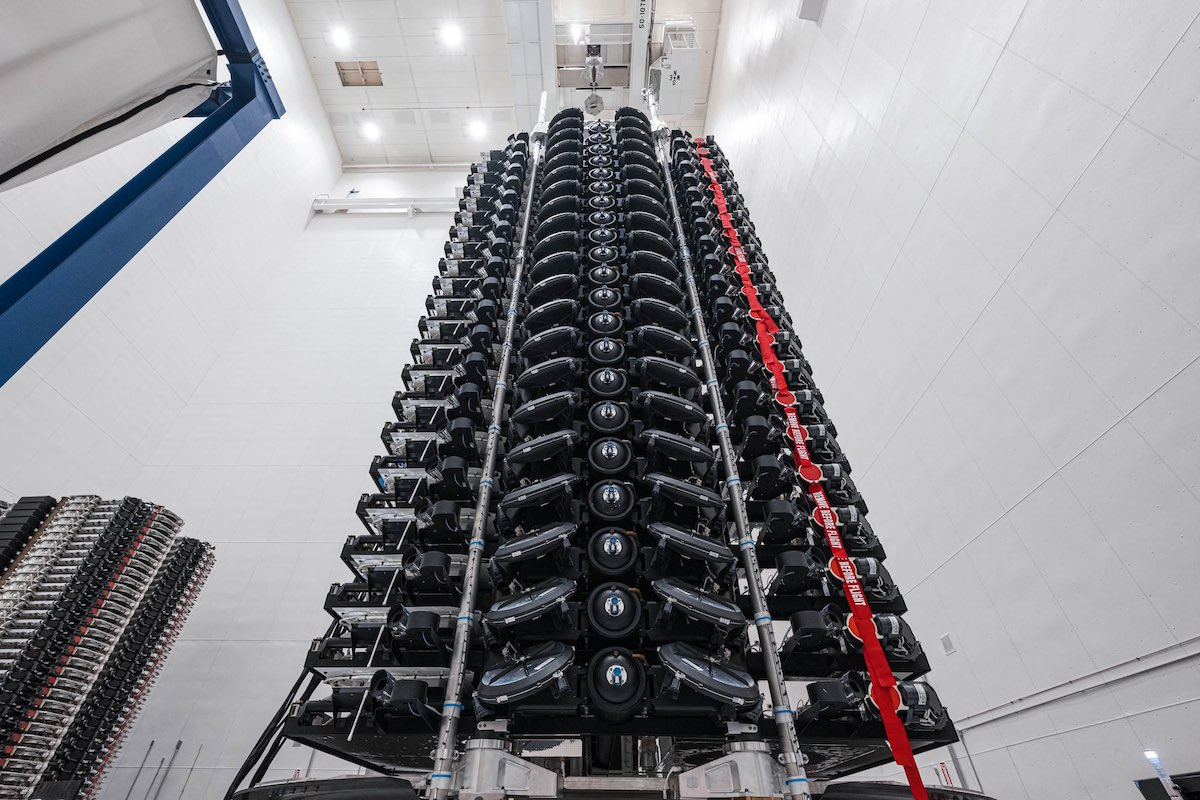
\includegraphics[width=0.7\linewidth]{./res/img/satellite_v2mini.jpg}
  \caption{Primo lotto dei satelliti "V2 Mini" pronto per il lancio in un razzo Falcon 9 da Cape Canaveral.}
  \label{fig:satellite_v2mini}
\end{figure}

Nel novembre 2024 SpaceX ha proposto una nuova iniziativa chiamata "Marslink", una versione adatta per Marte del suo sistema satellitare Starlink, per fornire servizi di trasmissione dati ad alta velocità tra Marte e la Terra. 
Il progetto, presentato a una riunione del NASA Mars Exploration Program Analysis Group, delinea l'utilizzo di satelliti in orbita attorno a Marte per garantire comunicazioni e supporto continui per le missioni di esplorazione.
Marslink mira a superare la velocità di trasmissione dati richiesta dalla NASA di 4 Mbps.
Questo sistema sfrutterebbe la tecnologica di comunicazione laser, consentendo il trasferimento di dati a lunga distanza attraverso le 1.5 unità astronomiche che separano Marte dal Sole \cite{michael_kan_spacex_2024}.

Starlink ha raggiunto 4 milioni di clienti a settembre 2024 \cite{starlink_starlink_nodate}.

\begin{figure}[htbp]
  \centering
  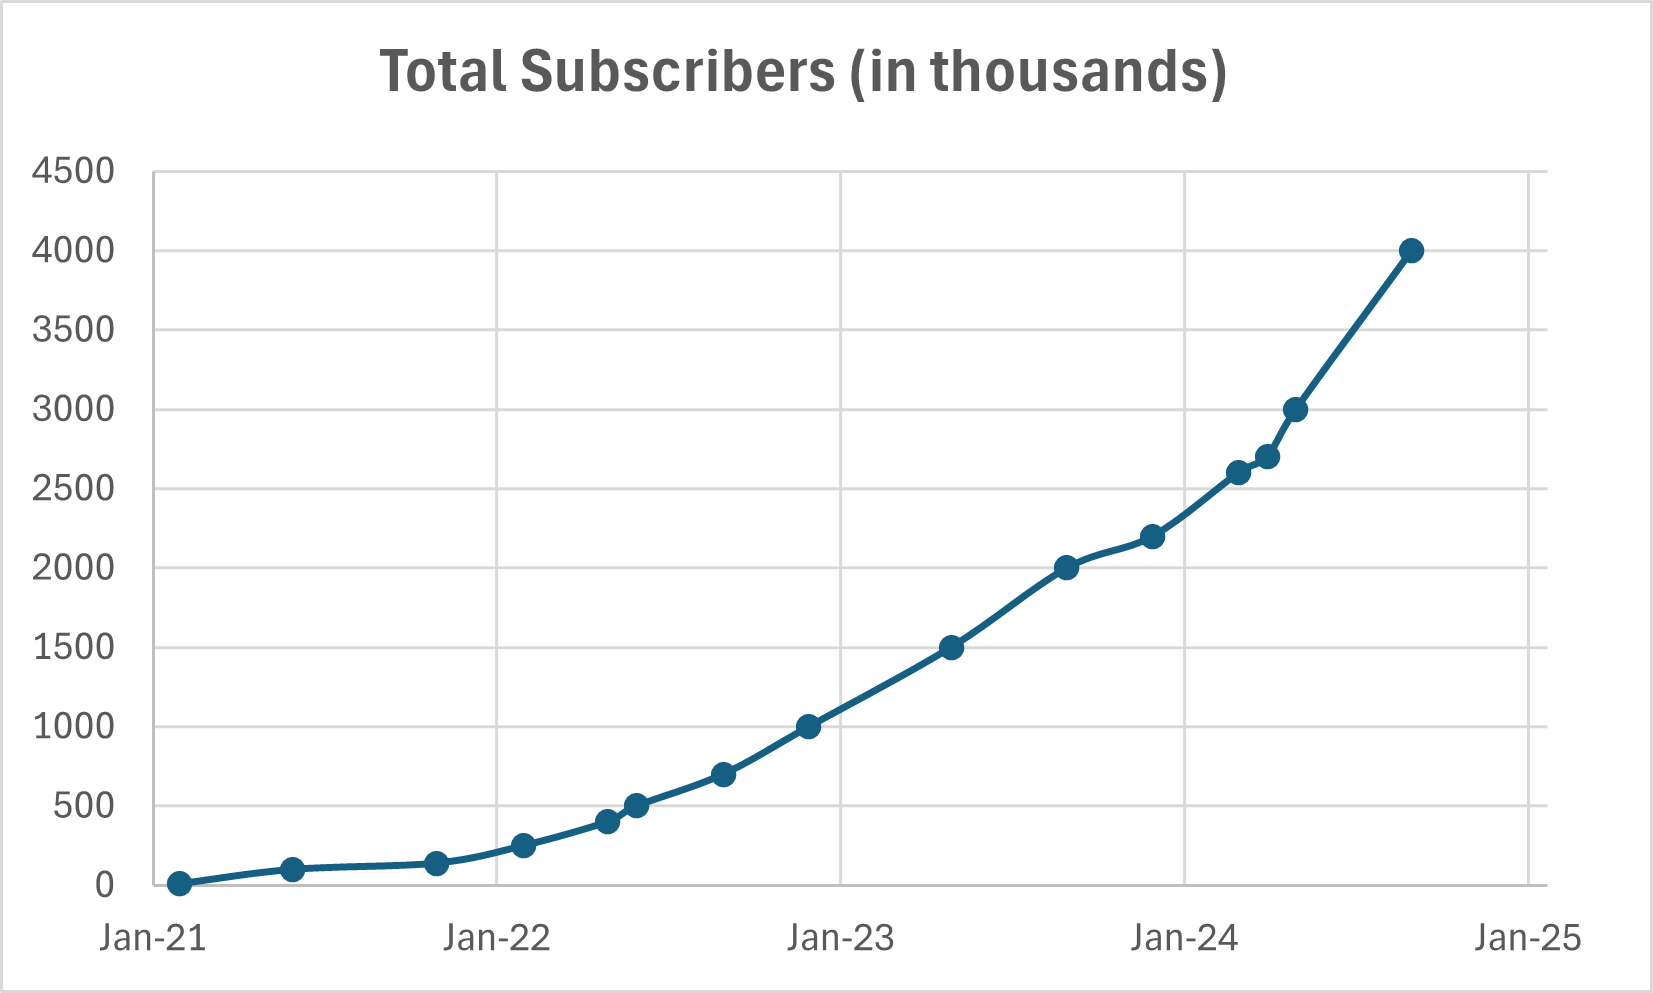
\includegraphics[width=0.7\linewidth]{./res/img/chart_subs.png}
  \caption{Numero di iscritti a Starlink}
  \label{fig:chart-subs}
\end{figure}

